
\subsection{Inference datasets: MNLI and HANS}
\label{sec:dataset}
MNLI~\citep{williams2017broad} is a popular NLU dataset containing more than 400,000 premise/hypothesis pairs annotated with textual entailment information (neutral, entailment or contradiction). Multiple studies have hypothesized that deep learning models tend to capture simple heuristics from the MNLI training data, and do not build an actual understanding of the task. Over the years, a series of diagnostic datasets have been released to test these hypotheses.
The most recent of these datasets, HANS~\citep[Heuristic Analysis for NLI Systems]{linzen2019right}, contains curated templates designed to test the robustness of a model against the following three heuristics for recognizing if a premise entails a hypothesis: lexical overlap (a premise entails any hypothesis built from a subset of its words), subsequence (a premise entails any of its contiguous subsequences) and constituent (a premise entails all the complete subtrees in its parse tree). In particular, any model relying exclusively on those heuristics would not have a higher than chance classification accuracy on this test set.

\citet{linzen2019right} show that a variety of existing models -- including BERT~\citep{devlin2018bert}, the state-of-the-art model at the time -- perform, overall, only slightly better than chance on classification accuracy of HANS evaluation data. This confirms the hypothesis that models trained on MNLI data tend to learn the three aforementioned heuristics rather than actually understanding the task. To test our methodology, we thus make use of the HANS evaluation dataset, which contains 30,000 examples equally split between the two labels: ``entailment'' and ``non-entailment''.\footnote{In HANS, ``contradiction'' and ``neutral'' labels are combined into ``non-entailment''.}

\subsection{Paraphrase datasets: QQP and PAWS}
\label{sec:dataset_qqp}

The QQP corpus~\citep{qqp} is another widely used NLU dataset containing over 400,000 pairs of sentences annotated as either paraphrase or non-paraphrase. As a consequence of the dataset design, pairs with high lexical overlap have a high probability of being paraphrases. Similarly to MNLI, models trained on QQP are thus prone to learning lexical overlap as a highly informative feature and do not capture the common sense underlying paraphrasing. 

In order to diagnose this phenomenon, \citet{zhang-etal-2019-paws} propose PAWS (Paraphrase Adversaries from Word Scrambling), a question paraphrase dataset containing over 108,000 sentence pairs well-balanced with respect to the word overlap heuristic. Models with high performance on QQP have been shown to perform terribly on PAWS' evaluation set: for example, the accuracy of BERT is around 91.3\% on QQP and only 32.2\% on PAWS (Table \ref{tab:paws}). This makes it an interesting test-bed for our method. 

In more details, PAWS has 2 sub-tasks, PAWS-wiki and PAWS-QQP. We use PAWS-QQP and report performance on its development set, which contains 677 questions pairs. To be comparable to results from~\citet{zhang-etal-2019-paws}, we reproduce the QQP split introduced by~\citet{wang2017bilateral} and we report results both in precision-recall area under the curve (AUC) and accuracy (Acc) (see Section \ref{sec:paws}). It is also important to note that the PAWS-QQP development set is not balanced. Training examples from PAWS were never used to update our models.



\subsection{Simple baselines for finding forgettables}
% as: here you need to restress that the simple baselines will serve as "bias models", i.e. we hope they will capture biases in the dataset and forgettable example will correspond to those example that do not match the biases (contribution of the paper basically)
We train two models, bag-of-words (BoW) and bidirectional LSTM (BiLSTM), as our simple baselines to compute forgetting statistics of different examples in the training set. We use the term \textit{simple} to emphasize the fact that these models have fewer parameters than the ones we will eventually consider (Section \ref{sec:strong}). Our conjecture is that networks with lower capacity will discover the samples that strongly support the various heuristics described in Sections \ref{sec:dataset} and  \ref{sec:dataset_qqp}. In particular, \emph{forgettable} examples for those models will correspond to sentences that do not verify said heuristics.

Both models are Siamese networks, with similar input representations and classification layers.
For the input layer, we lower case and tokenize the inputs into words and initialize their representations with Glove, a 300 dimensional pretrained embedding~\citep{pennington2014glove}.
For the classification task, from the premise and hypothesis vectors $p$ and $h$, we build the concatenated vector $s = [p, h, |p - h|, p \odot h]$ and pass it to a 2-layer feedforward network. 
To compute $p$ or $h$, the BoW model max-pools the bag of word embeddings,
while the BiLSTM model max-pools the top-layer hidden states of a 2-layer bidirectional LSTM. The hidden size of the LSTMs is set to 200. Overall, BoW and BiLSTM contains 560K and 2M parameters respectively.

\subsection{Target models}
\label{sec:strong}
Recently, significant improvements in many NLP tasks have been achieved by deep transformer-based models pretrained on huge amounts of unlabeled data.
Examples of such models include BERT \cite{devlin2018bert}, XLNET \cite{yang2019xlnet}, RoBERTA \cite{roberta2019}, AlBERT \cite{lan2019albert} and SpanBERT \cite{spanBERT2019}.
In this work, we focus on BERT and XLNET, both the base and large versions, and consider them as our strong models. In particular, \bertbase being the model of choice in previous work \cite{clark2019dont,zhang-etal-2019-paws}, it will serve as our default architecture.

\subsection{Computing forgetting events}
\label{sec:forg_stat}

We train our two simple baselines and \bertbase on MNLI and QQP
.We show the statistics of example forgetting in Table~\ref{tab:forg_stats}. The results below all make use of the balanced forgettable sets.

\begin{figure}[t]
\centering
  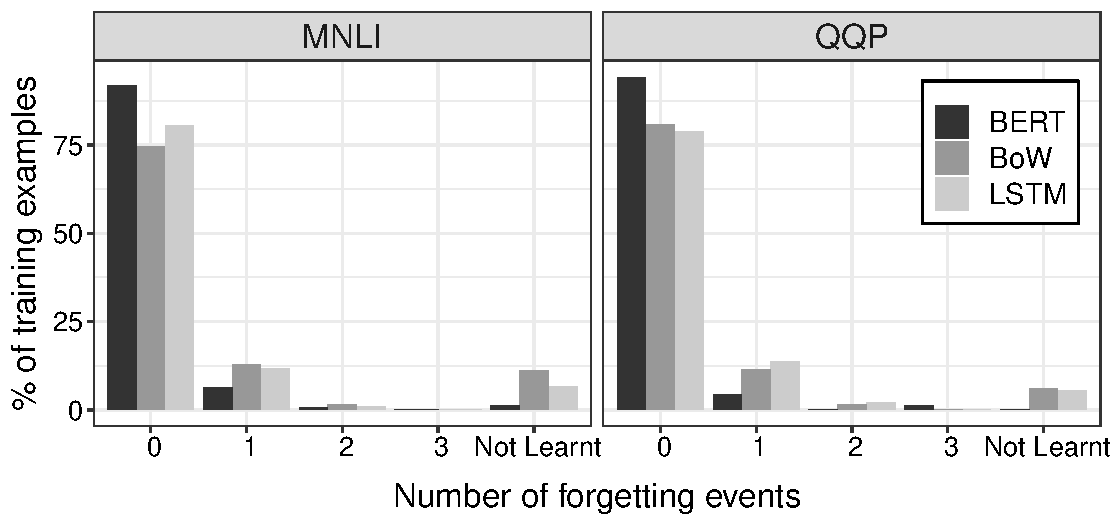
\includegraphics[width=0.48\textwidth]{figures/forgetting_counts.pdf}
  \caption{Distribution of forgetting events in MNLI and QQP training set for the three models after five training epochs. As can be seen, a majority of examples are not forgotten during training. We make use of examples 
  with at least one forgetting event in our method for robust models.}
\label{fig:forgcount-freq}
\end{figure}

Table \ref{tab:forg_stats} shows the number of forgettable examples before and after balancing for BoW, BiLSTM and BERT on MNLI. It is worth noting that the larger the model, the fewer the forgettable examples. The performance of the models on the dev set of MNLI is also included, and appears negatively correlated to the number of forgettable examples. Figure~\ref{fig:forgcount-freq} displays the distribution of forgetting events for each model on MNLI, showing in particular the significant number of examples never learnt by our simple baselines. We also see in Figure~\ref{fig:wordoverlap-unforg} that unforgettable examples have high (resp. low) word overlap in the entailment (resp. non-entailment) class. Example forgetting seems to correlate well with that known, strong heuristic.

Table \ref{tab:forg_stats} also contains the number of forgettable examples for our three default models on QQP. Interestingly, BiLSTM has more forgettables than BoW even though it reaches a better final performance. This fact could be explained by QQP having noisy labels, which has been shown to skew the number of forgetting events~\citep{toneva2018empirical}. The distribution of forgetting events for each model can be found in Figure \ref{fig:forgcount-freq}. In what follows, we denote the sets of forgettable examples from BERT, BiLSTM and BoW as \fbert, \flstm and \fbow  respectively.

\subsection{Fine-tuning on forgettable examples}
\label{sec:fine_tune}
We first fine-tune our target models on the whole dataset for $3$ epochs  to get a reasonable prior for the task. We then perform an additional stage of fine-tuning for $3$ epochs on a subset of the training set, composed of the forgettable examples from \fbert, \flstm or \fbow . 
